\documentclass{ocbeameruni}


\setdefaultlanguage[babelshorthands=true]{german}


% Nur benötigt für die Beispiel-Listings!
\usepackage{listings}
\lstloadlanguages{[LaTeX]TeX}
\lstset{%
  basicstyle=\small \ttfamily,
  breaklines=true,
}

\newcommand{\R}{\mathbb{R}}


\title{Organic Computing 2}
\subtitle{Lösungsvorschlag Blatt03}
\date{\today}
\author{Lukas Huhn \and Qiang Chang \and Victor Gerling}
\institute{%
  Universität Augsburg\\
  Institut für Informatik\\
  Lehrstuhl für Organic Computing
}


\begin{document}


\maketitle


\begin{frame}{Gliederung}
  \setbeamertemplate{section in toc}[sections numbered]
  \tableofcontents
\end{frame}


\section{Aufgabe 01}

\begin{frame}{Attribut City}
    \begin{itemize}
    \item Beispiele: 0, 1, 2(Cities sind mit 0 bis n durchnummeriert)
    \item n
    \end{itemize}
\end{frame}

\begin{frame}{Attribut Route}
    \begin{itemize}
    \item Beispiele: [(0,1),(1,2),(2,3),(3,0)], [(0,2), (2,1), (1,3), (3,0)], [(0,3), (3,1), (1,2), (2,0)]
    \item (n-1)!
    \end{itemize}
\end{frame}

\begin{frame}{Attribut Pheromone}
    \begin{itemize}
    \item Beispiele: 0.000002, 0.0002, 0.0000001
    \item Kontinierlicher Wertebereich, unendlich $\Rightarrow$ wir quantisieren! Wähle Minimum=0 und Maximum=0.0004 mit Step=1000
    $\Rightarrow$ 0.0000004 als Quantisierungsschritt
    \end{itemize}
\end{frame}

\begin{frame}{1.3 Routenlängen}
    \begin{center}
    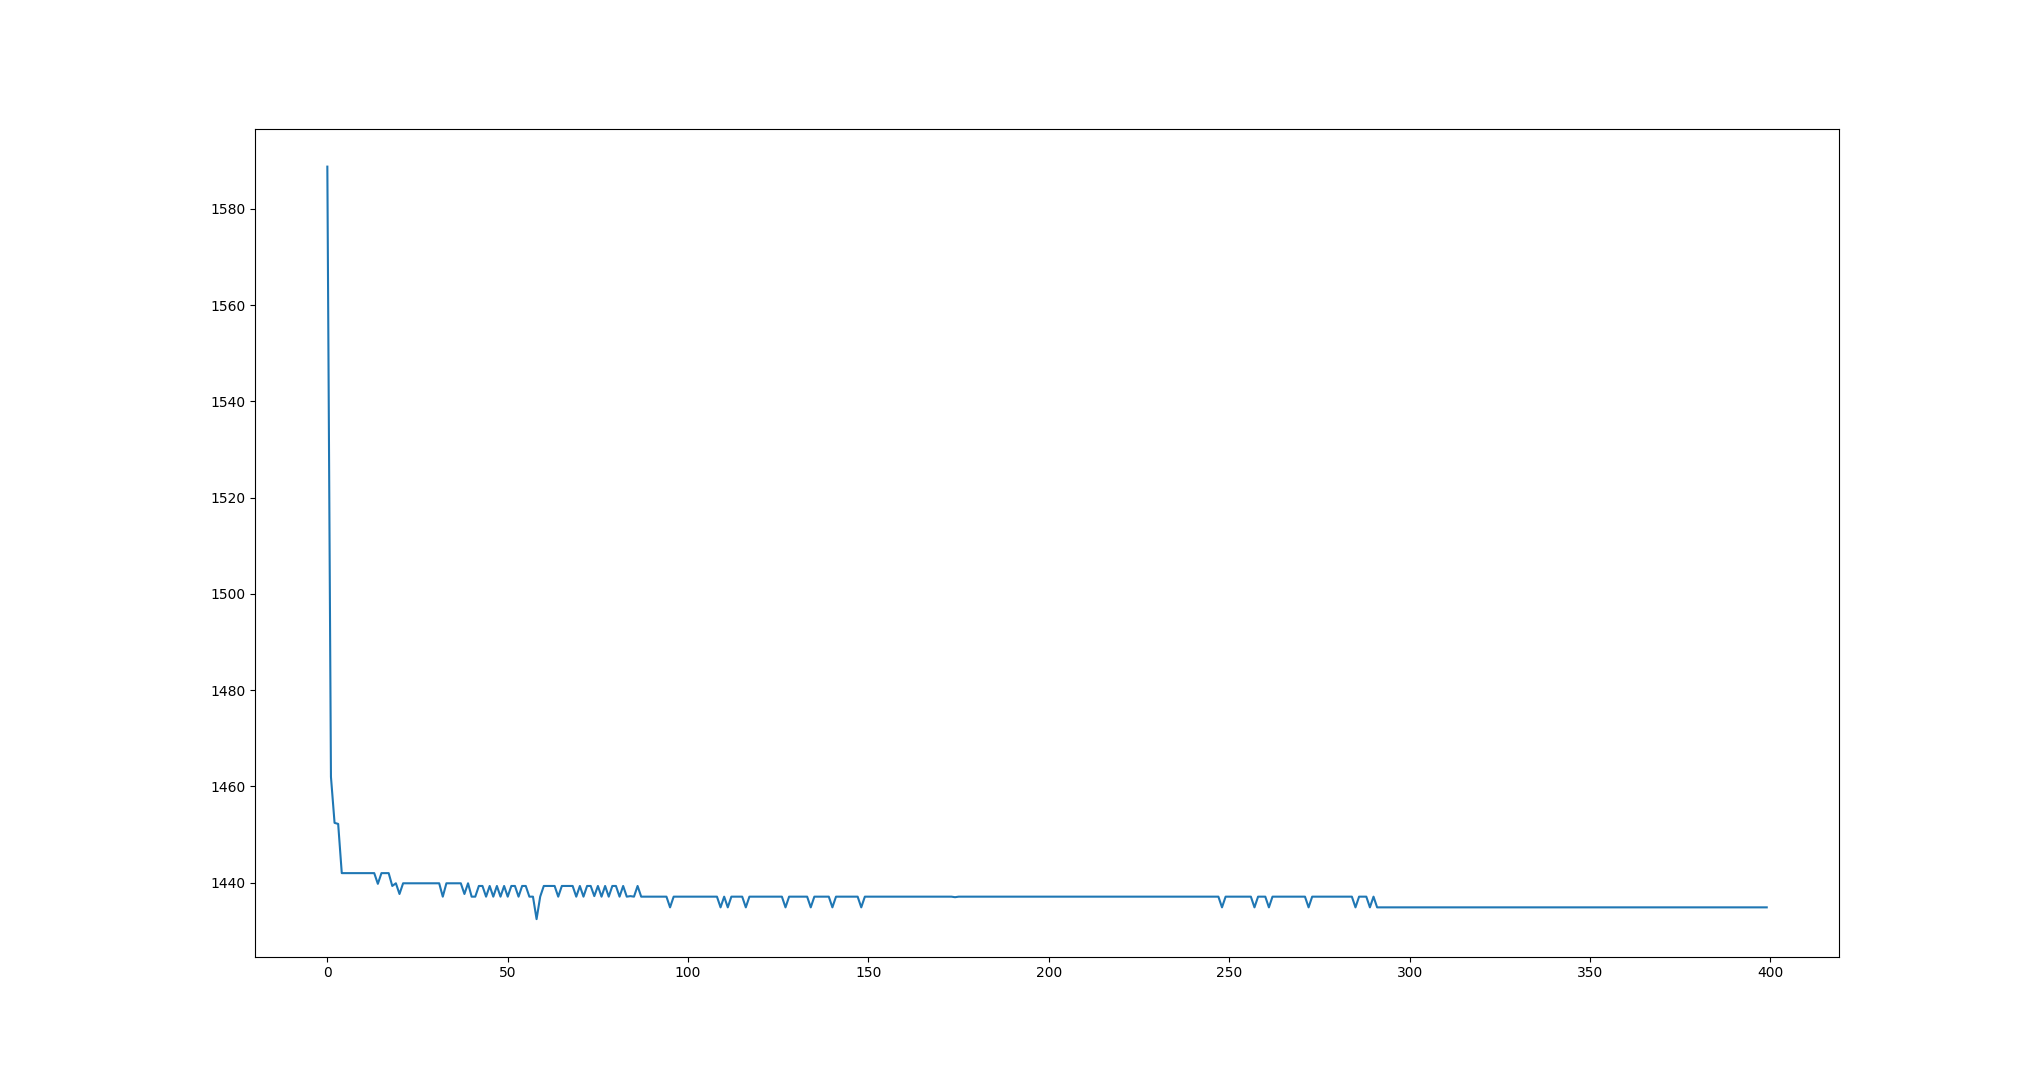
\includegraphics[scale=0.2]{Avg_len_per_iter.png}
    \end{center}
\end{frame}

\begin{frame}{1.3 Emergenz}
    \begin{center}
    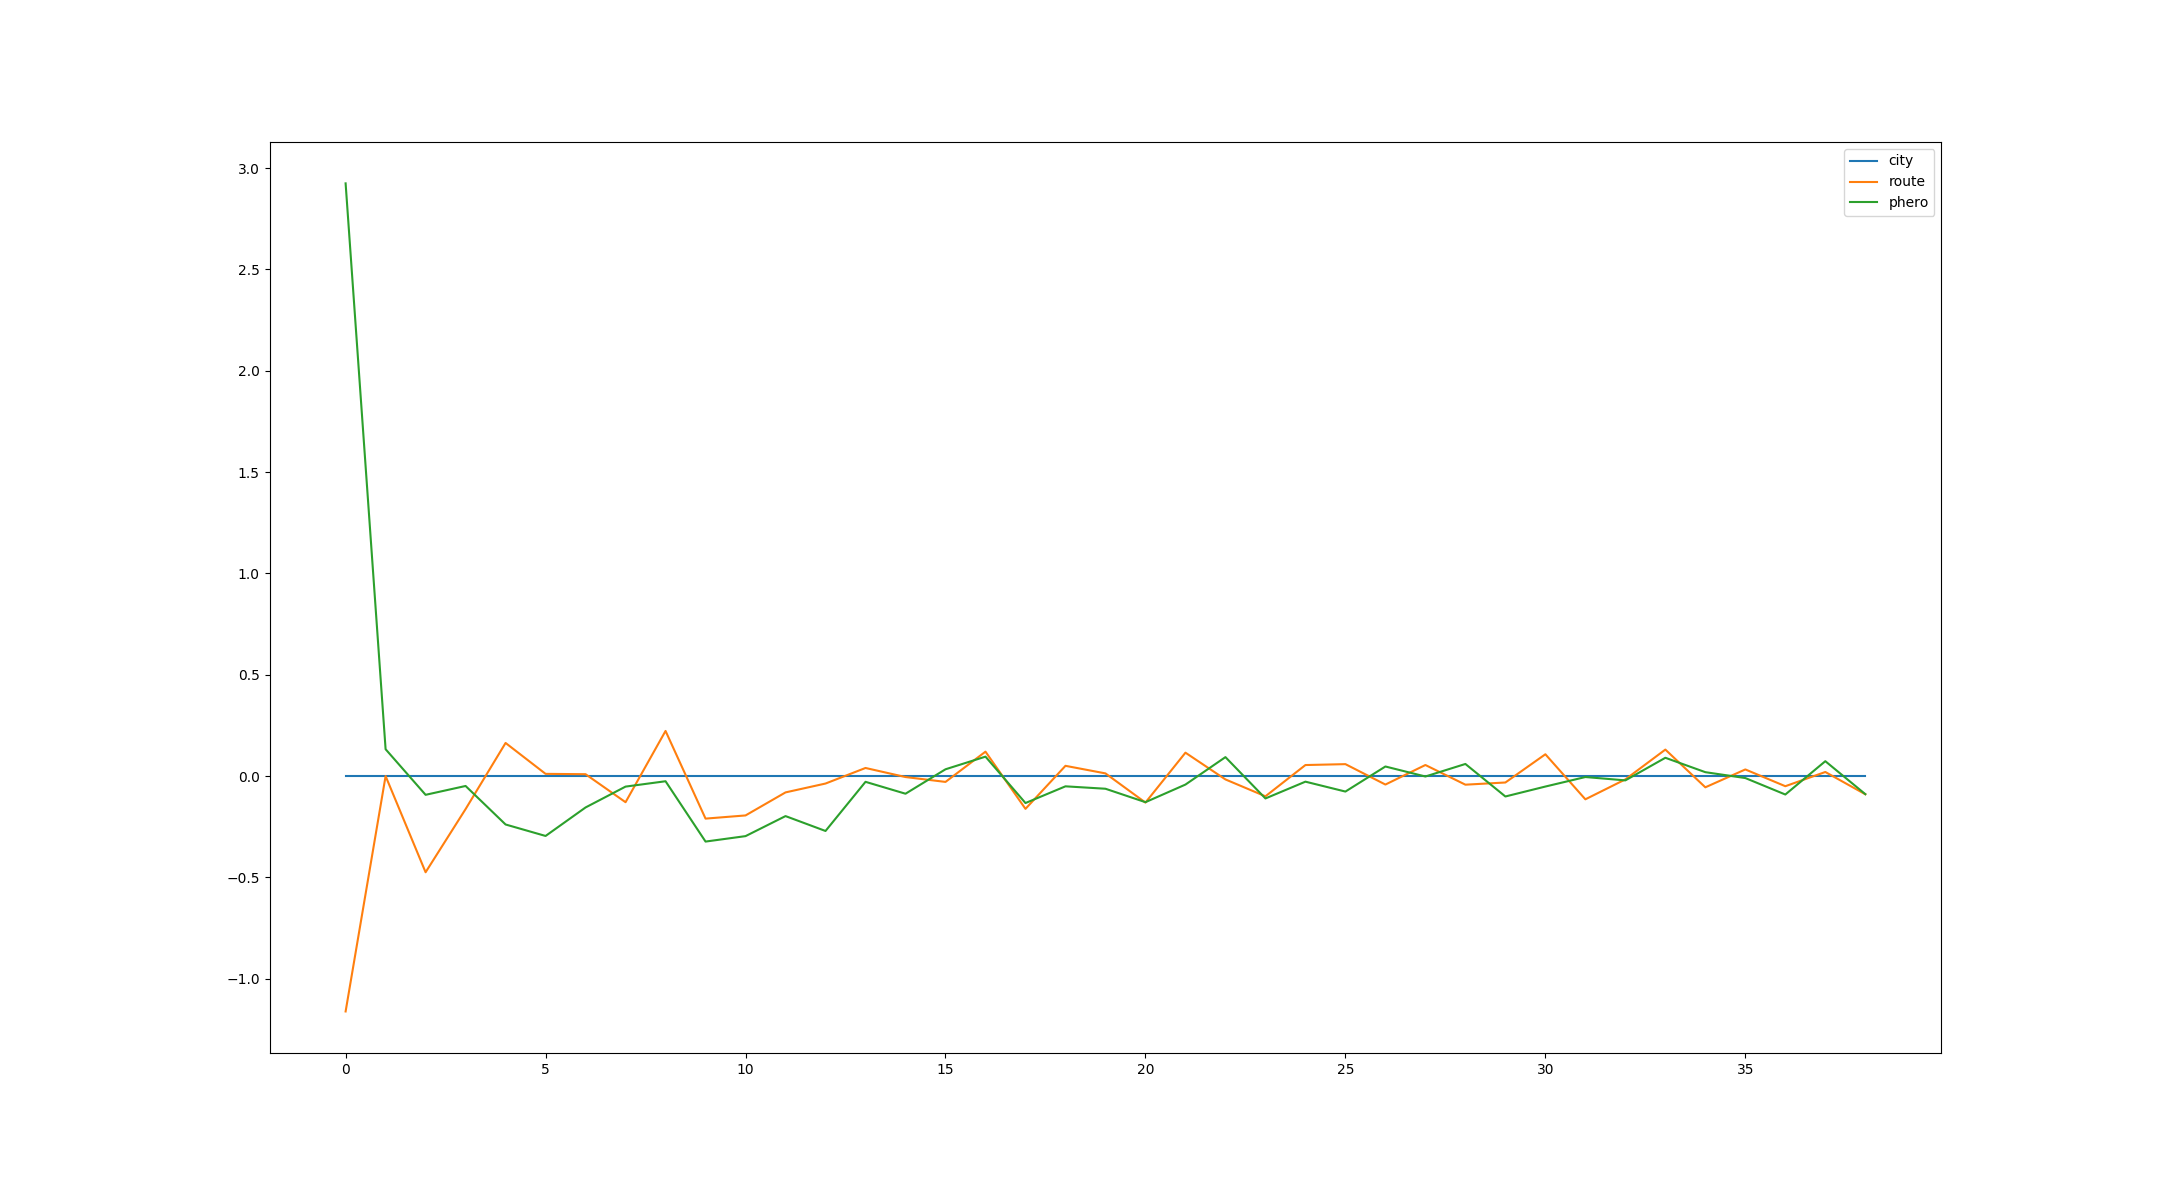
\includegraphics[scale=0.2]{Emerg_per_iter.png}
    \end{center}
\end{frame}

\begin{frame}{1.3 Emergenz Kiviat-Graph}
    \begin{center}
    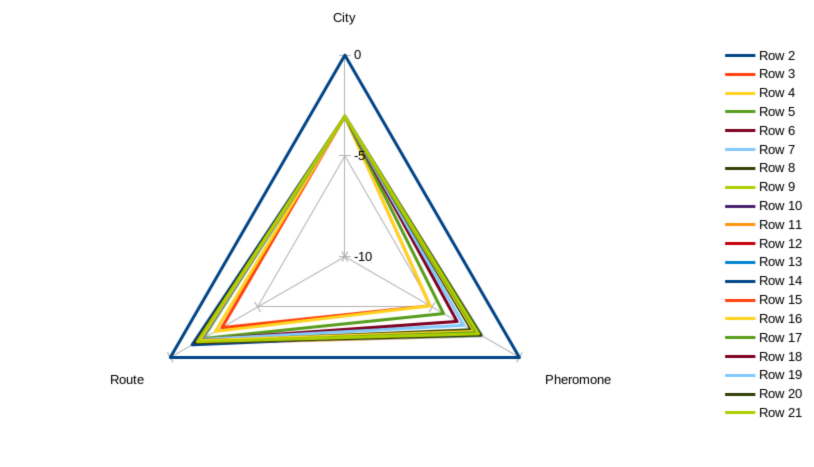
\includegraphics[scale=0.4]{emerg_spider.png}
    \end{center}
\end{frame}

\section{Aufgabe 04}

\begin{frame}{Emergenz vorhanden}
    \begin{itemize}
    \item Route: gut, weil sich Ants auf ähnliche Route einigen
    \item Pheromone: gut, weil sich mit der Zeit Pheromonenstärkste Straße herausbildet
    \end{itemize}
\end{frame}

\begin{frame}{Emergenz nicht vorhanden}
    \begin{itemize}
    \item City: Eventuell durch die verschiedenen Startstädte, ist jedoch eher weniger interessant
    \end{itemize}
\end{frame}


\end{document}
% Local Variables:
% TeX-engine: xetex
% End:
